\hypertarget{cli2_8cpp}{}\section{src/cli2.cpp File Reference}
\label{cli2_8cpp}\index{src/cli2.\+cpp@{src/cli2.\+cpp}}


Command line interface for hardware resource inspection.  


{\ttfamily \#include \char`\"{}cli2.\+hpp\char`\"{}}\newline
{\ttfamily \#include \char`\"{}sysinfo.\+hpp\char`\"{}}\newline
{\ttfamily \#include \char`\"{}top.\+hpp\char`\"{}}\newline
{\ttfamily \#include \char`\"{}threadinfo.\+hpp\char`\"{}}\newline
{\ttfamily \#include \char`\"{}cli\+\_\+appereance.\+hpp\char`\"{}}\newline
Include dependency graph for cli2.\+cpp\+:\nopagebreak
\begin{figure}[H]
\begin{center}
\leavevmode
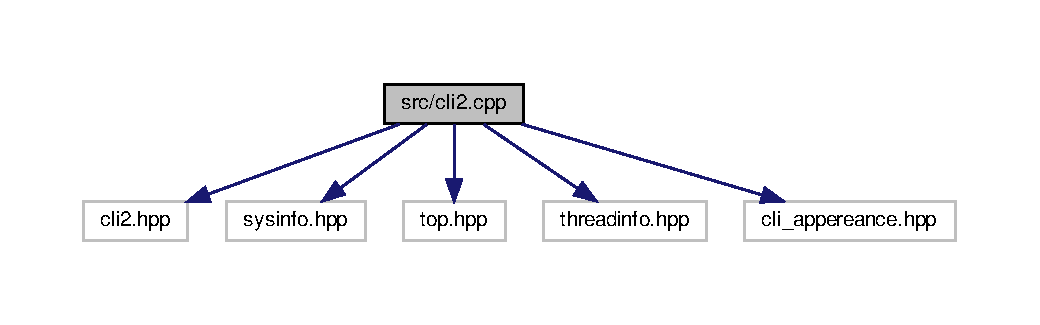
\includegraphics[width=350pt]{cli2_8cpp__incl}
\end{center}
\end{figure}


\subsection{Detailed Description}
Command line interface for hardware resource inspection. 

The command line interface (cli) allows the developer to check the C\+PU and memory usage, the number of active threads and display the main variables. The available commands are\+:
\begin{DoxyItemize}
\item top Display C\+PU usage;
\item info Display hardware information;
\item thread Show active threads state, priority and their resources;
\item clear Clear screen;
\item help Show available commands. 
\end{DoxyItemize}